\section{Vorgehen}
\begin{enumerate}
\item Gewähltes Problem aus dem Katalog von Karp notieren
\item Reduktion des gegebenen Problems, auf das bekannte aus Karp
\item Beschreibung der Reduktion
\item Schlussfolgerung: Da das Problem aus dem Katalog von Karp NP-vollständig ist, gibt es auch keinen effizienten (polynomiellen) Algorithmus, der das gegebene Problem lösen könnte.
\end{enumerate}
Schlusssatz:
Dies ist genau die Beschreibung des Problems HMMM. Das Problem HMMM ist NP-vollständig, nach aktuellem Wissen gibt es also keinen effizienten (polynomiellen) Algorithmus, der ein HMMM Problem lösen könnte.

Manchmal ist es schwierig SET-COVERING, EXACT-COVER und SET-PACKING auseinander
zu halten. Man beachte:
- In SET-COVERING und in SET-PACKING kommt eine Zahl k vor, nicht aber in EXACT-
COVER.
- In SET-COVERING dürfen sich die Mengen schneiden, müssen aber auch alles abdecken.
In SET-PACKING dürfen sich die Mengen nicht schneiden, müssen aber auch nicht alles
abdecken.
- In EXACT-COVER dürfen sich die Mengen nicht schneiden, müssen alles abdecken, aber
es kommt nicht auf ihre Anzahl an.

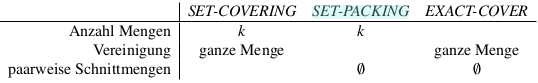
\includegraphics[width=\columnwidth]{img/setvscoveringvsexact.png}